\documentclass[a4paper, 12pt]{article}


\usepackage{amsmath,amssymb,amsthm,bm} % 数学符号和公式
\usepackage{tikz}  % 绘图包
\usepackage{xcolor} % 用于给超链接指定颜色
\usepackage{float} % 浮动体
\usepackage{graphics} % 插入图片

\usepackage{geometry} % 页边距
\geometry{top=3cm,bottom=3cm,left=2.5cm,right=2.5cm}

\usepackage{fancyhdr} % 页眉页脚设置
\usepackage{lastpage}
\fancypagestyle{plain}{%
    \fancyhf{} % 清空所有预设样式
    \fancyfoot[C]{\thepage{}/\pageref*{LastPage}} % 设置页脚中心位置
    \renewcommand{\headrulewidth}{0.4pt} % 页眉横线的宽度
    \renewcommand{\footrulewidth}{0pt}   % 页脚横线的宽度
}
\pagestyle{plain}

\usepackage{booktabs} % 表格
\setlength{\arrayrulewidth}{0.08em} % 普通表格的线宽
\usepackage[flushleft]{threeparttable } % 表格下方的说明
\usepackage{tabularx} % 环境tabularx, 自动计算表格列宽
\newcolumntype{Y}{>{\centering\arraybackslash}X} % 居中排列, 且自动计算列宽
\usepackage{tabularray} % 表格环境, 网页导出的表格的要求
\usepackage[flushleft]{threeparttable} % 表格下边的脚注, 靠左对齐
\usepackage{caption}  % 图例
\usepackage{setspace} % 空白
% ---------------- Pdf_latex From Inkscape --------------- %
% 用于插入inkscape生成的带有latex标注的图片
\usepackage{import}
\graphicspath{{./figure}} % 声明 pdf_tex和对应pdf所在的文件夹
\usepackage{xifthen}
\usepackage{pdfpages}
\usepackage{transparent}
% -------------------------------------------------------- %
\usepackage{hyperref} % 超链接格式
\usepackage{fixdif} % 积分符号\d
\usepackage[noabbrev]{cleveref} % 交叉引用
% 颜色设置要在cleveref包之后
\def\mycolor{purple}
\hypersetup{colorlinks=true,linkcolor=\mycolor,citecolor=\mycolor,urlcolor=\mycolor}
\usepackage{apacite}
\usepackage{natbib}
\begin{document}

\begin{titlepage}
    \title{A Title for This Paper\thanks{abc}}
    % 作者和作者简介
    \author{XJZ\thanks{USTC} \and WLZ\thanks{CPU}}
    \date{\today}
    \maketitle
    \begin{abstract}
        \noindent
        % 摘要
        This is you abstract.
        \\
        \vspace{0in}\\
        % 关键字
        \noindent\textbf{Keywords:} climate, AI, robots\\
        \bigskip
    \end{abstract}
    \setcounter{page}{0}
    \thispagestyle{empty}
\end{titlepage}
\pagebreak \newpage
\doublespacing

\section{Introduction}\label{sec:intro}
Parentheses citation \citep{DunningHuchetteLubin2017}, and author-year citation \citet{DunningHuchetteLubin2017}, cite a book \citep[\S 2.1.1]{DunningHuchetteLubin2017}

% \Cref{} 可以用于表格、图片、章节的交叉引用, 不可用于参考文献
ref you section \Cref{sec:intro}
\begin{figure}[!htbp]
    \centering
    % 这里导入的tikz要通过vsc的httpgd浏览器导出, 450 * 300, tikz可以保证最后字体和正文字体一致,字号和ggplot2指定的一致
    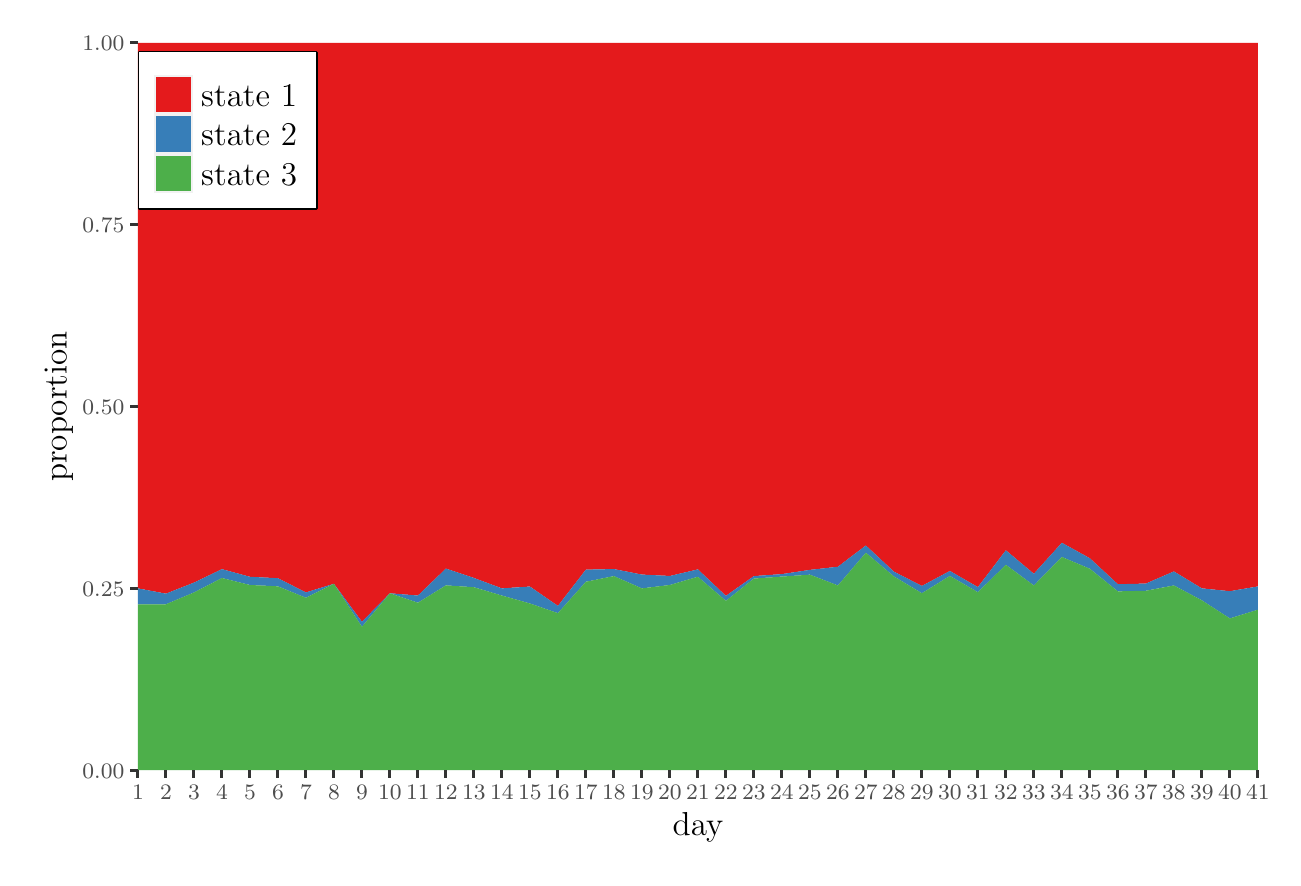
\begin{tikzpicture}[x=1pt,y=-1pt,scale=1.00]
\fill[fill={rgb,255:red,255; green,255; blue,255}] (0,0) rectangle (450.00,300.00);
\begin{scope}\clip (0.00,0.00) rectangle (450.00,300.00);
\draw[fill={rgb,255:red,255; green,255; blue,255},line width=1.07pt,draw={rgb,255:red,255; green,255; blue,255},line cap=round,line join=round] (0.00,0.00) rectangle (450.00,300.00);
\end{scope}\begin{scope}\clip (39.84,5.48) rectangle (444.52,268.32);
\draw[fill={rgb,255:red,235; green,235; blue,235},line width=1.07pt,draw=none,line cap=round,line join=round] (39.84,5.48) rectangle (444.52,268.32);
\draw[line width=0.53pt,draw={rgb,255:red,255; green,255; blue,255},line join=round] (39.84,235.46) -- (444.52,235.46);
\draw[line width=0.53pt,draw={rgb,255:red,255; green,255; blue,255},line join=round] (39.84,169.75) -- (444.52,169.75);
\draw[line width=0.53pt,draw={rgb,255:red,255; green,255; blue,255},line join=round] (39.84,104.04) -- (444.52,104.04);
\draw[line width=0.53pt,draw={rgb,255:red,255; green,255; blue,255},line join=round] (39.84,38.33) -- (444.52,38.33);
\draw[line width=1.07pt,draw={rgb,255:red,255; green,255; blue,255},line join=round] (39.84,268.32) -- (444.52,268.32);
\draw[line width=1.07pt,draw={rgb,255:red,255; green,255; blue,255},line join=round] (39.84,202.61) -- (444.52,202.61);
\draw[line width=1.07pt,draw={rgb,255:red,255; green,255; blue,255},line join=round] (39.84,136.90) -- (444.52,136.90);
\draw[line width=1.07pt,draw={rgb,255:red,255; green,255; blue,255},line join=round] (39.84,71.19) -- (444.52,71.19);
\draw[line width=1.07pt,draw={rgb,255:red,255; green,255; blue,255},line join=round] (39.84,5.48) -- (444.52,5.48);
\draw[line width=1.07pt,draw={rgb,255:red,255; green,255; blue,255},line join=round] (39.84,268.32) -- (39.84,5.48);
\draw[line width=1.07pt,draw={rgb,255:red,255; green,255; blue,255},line join=round] (49.96,268.32) -- (49.96,5.48);
\draw[line width=1.07pt,draw={rgb,255:red,255; green,255; blue,255},line join=round] (60.08,268.32) -- (60.08,5.48);
\draw[line width=1.07pt,draw={rgb,255:red,255; green,255; blue,255},line join=round] (70.19,268.32) -- (70.19,5.48);
\draw[line width=1.07pt,draw={rgb,255:red,255; green,255; blue,255},line join=round] (80.31,268.32) -- (80.31,5.48);
\draw[line width=1.07pt,draw={rgb,255:red,255; green,255; blue,255},line join=round] (90.43,268.32) -- (90.43,5.48);
\draw[line width=1.07pt,draw={rgb,255:red,255; green,255; blue,255},line join=round] (100.54,268.32) -- (100.54,5.48);
\draw[line width=1.07pt,draw={rgb,255:red,255; green,255; blue,255},line join=round] (110.66,268.32) -- (110.66,5.48);
\draw[line width=1.07pt,draw={rgb,255:red,255; green,255; blue,255},line join=round] (120.78,268.32) -- (120.78,5.48);
\draw[line width=1.07pt,draw={rgb,255:red,255; green,255; blue,255},line join=round] (130.89,268.32) -- (130.89,5.48);
\draw[line width=1.07pt,draw={rgb,255:red,255; green,255; blue,255},line join=round] (141.01,268.32) -- (141.01,5.48);
\draw[line width=1.07pt,draw={rgb,255:red,255; green,255; blue,255},line join=round] (151.13,268.32) -- (151.13,5.48);
\draw[line width=1.07pt,draw={rgb,255:red,255; green,255; blue,255},line join=round] (161.24,268.32) -- (161.24,5.48);
\draw[line width=1.07pt,draw={rgb,255:red,255; green,255; blue,255},line join=round] (171.36,268.32) -- (171.36,5.48);
\draw[line width=1.07pt,draw={rgb,255:red,255; green,255; blue,255},line join=round] (181.48,268.32) -- (181.48,5.48);
\draw[line width=1.07pt,draw={rgb,255:red,255; green,255; blue,255},line join=round] (191.60,268.32) -- (191.60,5.48);
\draw[line width=1.07pt,draw={rgb,255:red,255; green,255; blue,255},line join=round] (201.71,268.32) -- (201.71,5.48);
\draw[line width=1.07pt,draw={rgb,255:red,255; green,255; blue,255},line join=round] (211.83,268.32) -- (211.83,5.48);
\draw[line width=1.07pt,draw={rgb,255:red,255; green,255; blue,255},line join=round] (221.95,268.32) -- (221.95,5.48);
\draw[line width=1.07pt,draw={rgb,255:red,255; green,255; blue,255},line join=round] (232.06,268.32) -- (232.06,5.48);
\draw[line width=1.07pt,draw={rgb,255:red,255; green,255; blue,255},line join=round] (242.18,268.32) -- (242.18,5.48);
\draw[line width=1.07pt,draw={rgb,255:red,255; green,255; blue,255},line join=round] (252.30,268.32) -- (252.30,5.48);
\draw[line width=1.07pt,draw={rgb,255:red,255; green,255; blue,255},line join=round] (262.41,268.32) -- (262.41,5.48);
\draw[line width=1.07pt,draw={rgb,255:red,255; green,255; blue,255},line join=round] (272.53,268.32) -- (272.53,5.48);
\draw[line width=1.07pt,draw={rgb,255:red,255; green,255; blue,255},line join=round] (282.65,268.32) -- (282.65,5.48);
\draw[line width=1.07pt,draw={rgb,255:red,255; green,255; blue,255},line join=round] (292.77,268.32) -- (292.77,5.48);
\draw[line width=1.07pt,draw={rgb,255:red,255; green,255; blue,255},line join=round] (302.88,268.32) -- (302.88,5.48);
\draw[line width=1.07pt,draw={rgb,255:red,255; green,255; blue,255},line join=round] (313.00,268.32) -- (313.00,5.48);
\draw[line width=1.07pt,draw={rgb,255:red,255; green,255; blue,255},line join=round] (323.12,268.32) -- (323.12,5.48);
\draw[line width=1.07pt,draw={rgb,255:red,255; green,255; blue,255},line join=round] (333.23,268.32) -- (333.23,5.48);
\draw[line width=1.07pt,draw={rgb,255:red,255; green,255; blue,255},line join=round] (343.35,268.32) -- (343.35,5.48);
\draw[line width=1.07pt,draw={rgb,255:red,255; green,255; blue,255},line join=round] (353.47,268.32) -- (353.47,5.48);
\draw[line width=1.07pt,draw={rgb,255:red,255; green,255; blue,255},line join=round] (363.58,268.32) -- (363.58,5.48);
\draw[line width=1.07pt,draw={rgb,255:red,255; green,255; blue,255},line join=round] (373.70,268.32) -- (373.70,5.48);
\draw[line width=1.07pt,draw={rgb,255:red,255; green,255; blue,255},line join=round] (383.82,268.32) -- (383.82,5.48);
\draw[line width=1.07pt,draw={rgb,255:red,255; green,255; blue,255},line join=round] (393.94,268.32) -- (393.94,5.48);
\draw[line width=1.07pt,draw={rgb,255:red,255; green,255; blue,255},line join=round] (404.05,268.32) -- (404.05,5.48);
\draw[line width=1.07pt,draw={rgb,255:red,255; green,255; blue,255},line join=round] (414.17,268.32) -- (414.17,5.48);
\draw[line width=1.07pt,draw={rgb,255:red,255; green,255; blue,255},line join=round] (424.29,268.32) -- (424.29,5.48);
\draw[line width=1.07pt,draw={rgb,255:red,255; green,255; blue,255},line join=round] (434.40,268.32) -- (434.40,5.48);
\draw[line width=1.07pt,draw={rgb,255:red,255; green,255; blue,255},line join=round] (444.52,268.32) -- (444.52,5.48);
\draw[fill={rgb,255:red,228; green,26; blue,28},line width=0.00pt,draw=none,line cap=round,line join=round] (39.84,5.48) -- (49.96,5.48) -- (60.08,5.48) -- (70.19,5.48) -- (80.31,5.48) -- (90.43,5.48) -- (100.54,5.48) -- (110.66,5.48) -- (120.78,5.48) -- (130.89,5.48) -- (141.01,5.48) -- (151.13,5.48) -- (161.24,5.48) -- (171.36,5.48) -- (181.48,5.48) -- (191.60,5.48) -- (201.71,5.48) -- (211.83,5.48) -- (221.95,5.48) -- (232.06,5.48) -- (242.18,5.48) -- (252.30,5.48) -- (262.41,5.48) -- (272.53,5.48) -- (282.65,5.48) -- (292.77,5.48) -- (302.88,5.48) -- (313.00,5.48) -- (323.12,5.48) -- (333.23,5.48) -- (343.35,5.48) -- (353.47,5.48) -- (363.58,5.48) -- (373.70,5.48) -- (383.82,5.48) -- (393.94,5.48) -- (404.05,5.48) -- (414.17,5.48) -- (424.29,5.48) -- (434.40,5.48) -- (444.52,5.48) -- (444.52,201.91) -- (434.40,203.63) -- (424.29,202.61) -- (414.17,196.48) -- (404.05,200.88) -- (393.94,201.10) -- (383.82,191.73) -- (373.70,186.13) -- (363.58,197.33) -- (353.47,188.85) -- (343.35,202.15) -- (333.23,196.31) -- (323.12,201.73) -- (313.00,196.56) -- (302.88,187.11) -- (292.77,194.79) -- (282.65,195.93) -- (272.53,197.45) -- (262.41,198.17) -- (252.30,205.31) -- (242.18,195.75) -- (232.06,198.12) -- (221.95,197.62) -- (211.83,195.63) -- (201.71,195.84) -- (191.60,208.94) -- (181.48,201.95) -- (171.36,202.61) -- (161.24,198.84) -- (151.13,195.45) -- (141.01,205.20) -- (130.89,204.38) -- (120.78,214.66) -- (110.66,200.95) -- (100.54,204.07) -- (90.43,198.94) -- (80.31,198.42) -- (70.19,195.66) -- (60.08,200.53) -- (49.96,204.52) -- (39.84,202.61) -- cycle;
\draw[line width=1.07pt,draw=none,line cap=round,line join=round] (39.84,5.48) -- (49.96,5.48) -- (60.08,5.48) -- (70.19,5.48) -- (80.31,5.48) -- (90.43,5.48) -- (100.54,5.48) -- (110.66,5.48) -- (120.78,5.48) -- (130.89,5.48) -- (141.01,5.48) -- (151.13,5.48) -- (161.24,5.48) -- (171.36,5.48) -- (181.48,5.48) -- (191.60,5.48) -- (201.71,5.48) -- (211.83,5.48) -- (221.95,5.48) -- (232.06,5.48) -- (242.18,5.48) -- (252.30,5.48) -- (262.41,5.48) -- (272.53,5.48) -- (282.65,5.48) -- (292.77,5.48) -- (302.88,5.48) -- (313.00,5.48) -- (323.12,5.48) -- (333.23,5.48) -- (343.35,5.48) -- (353.47,5.48) -- (363.58,5.48) -- (373.70,5.48) -- (383.82,5.48) -- (393.94,5.48) -- (404.05,5.48) -- (414.17,5.48) -- (424.29,5.48) -- (434.40,5.48) -- (444.52,5.48);
\draw[fill={rgb,255:red,55; green,126; blue,184},line width=0.00pt,draw=none,line cap=round,line join=round] (39.84,202.61) -- (49.96,204.52) -- (60.08,200.53) -- (70.19,195.66) -- (80.31,198.42) -- (90.43,198.94) -- (100.54,204.07) -- (110.66,200.95) -- (120.78,214.66) -- (130.89,204.38) -- (141.01,205.20) -- (151.13,195.45) -- (161.24,198.84) -- (171.36,202.61) -- (181.48,201.95) -- (191.60,208.94) -- (201.71,195.84) -- (211.83,195.63) -- (221.95,197.62) -- (232.06,198.12) -- (242.18,195.75) -- (252.30,205.31) -- (262.41,198.17) -- (272.53,197.45) -- (282.65,195.93) -- (292.77,194.79) -- (302.88,187.11) -- (313.00,196.56) -- (323.12,201.73) -- (333.23,196.31) -- (343.35,202.15) -- (353.47,188.85) -- (363.58,197.33) -- (373.70,186.13) -- (383.82,191.73) -- (393.94,201.10) -- (404.05,200.88) -- (414.17,196.48) -- (424.29,202.61) -- (434.40,203.63) -- (444.52,201.91) -- (444.52,210.32) -- (434.40,213.46) -- (424.29,206.93) -- (414.17,201.55) -- (404.05,203.47) -- (393.94,203.68) -- (383.82,195.52) -- (373.70,191.26) -- (363.58,201.55) -- (353.47,194.09) -- (343.35,203.99) -- (333.23,198.11) -- (323.12,204.36) -- (313.00,198.28) -- (302.88,189.73) -- (292.77,201.55) -- (282.65,197.65) -- (272.53,198.35) -- (262.41,199.06) -- (252.30,207.11) -- (242.18,198.40) -- (232.06,201.38) -- (221.95,202.61) -- (211.83,198.17) -- (201.71,200.21) -- (191.60,211.56) -- (181.48,208.06) -- (171.36,205.20) -- (161.24,202.19) -- (151.13,201.52) -- (141.01,207.79) -- (130.89,204.38) -- (120.78,216.48) -- (110.66,200.95) -- (100.54,206.01) -- (90.43,201.87) -- (80.31,201.38) -- (70.19,198.87) -- (60.08,204.09) -- (49.96,208.35) -- (39.84,208.41) -- cycle;
\draw[line width=1.07pt,draw=none,line cap=round,line join=round] (39.84,202.61) -- (49.96,204.52) -- (60.08,200.53) -- (70.19,195.66) -- (80.31,198.42) -- (90.43,198.94) -- (100.54,204.07) -- (110.66,200.95) -- (120.78,214.66) -- (130.89,204.38) -- (141.01,205.20) -- (151.13,195.45) -- (161.24,198.84) -- (171.36,202.61) -- (181.48,201.95) -- (191.60,208.94) -- (201.71,195.84) -- (211.83,195.63) -- (221.95,197.62) -- (232.06,198.12) -- (242.18,195.75) -- (252.30,205.31) -- (262.41,198.17) -- (272.53,197.45) -- (282.65,195.93) -- (292.77,194.79) -- (302.88,187.11) -- (313.00,196.56) -- (323.12,201.73) -- (333.23,196.31) -- (343.35,202.15) -- (353.47,188.85) -- (363.58,197.33) -- (373.70,186.13) -- (383.82,191.73) -- (393.94,201.10) -- (404.05,200.88) -- (414.17,196.48) -- (424.29,202.61) -- (434.40,203.63) -- (444.52,201.91);
\draw[fill={rgb,255:red,77; green,175; blue,74},line width=0.00pt,draw=none,line cap=round,line join=round] (39.84,208.41) -- (49.96,208.35) -- (60.08,204.09) -- (70.19,198.87) -- (80.31,201.38) -- (90.43,201.87) -- (100.54,206.01) -- (110.66,200.95) -- (120.78,216.48) -- (130.89,204.38) -- (141.01,207.79) -- (151.13,201.52) -- (161.24,202.19) -- (171.36,205.20) -- (181.48,208.06) -- (191.60,211.56) -- (201.71,200.21) -- (211.83,198.17) -- (221.95,202.61) -- (232.06,201.38) -- (242.18,198.40) -- (252.30,207.11) -- (262.41,199.06) -- (272.53,198.35) -- (282.65,197.65) -- (292.77,201.55) -- (302.88,189.73) -- (313.00,198.28) -- (323.12,204.36) -- (333.23,198.11) -- (343.35,203.99) -- (353.47,194.09) -- (363.58,201.55) -- (373.70,191.26) -- (383.82,195.52) -- (393.94,203.68) -- (404.05,203.47) -- (414.17,201.55) -- (424.29,206.93) -- (434.40,213.46) -- (444.52,210.32) -- (444.52,268.32) -- (434.40,268.32) -- (424.29,268.32) -- (414.17,268.32) -- (404.05,268.32) -- (393.94,268.32) -- (383.82,268.32) -- (373.70,268.32) -- (363.58,268.32) -- (353.47,268.32) -- (343.35,268.32) -- (333.23,268.32) -- (323.12,268.32) -- (313.00,268.32) -- (302.88,268.32) -- (292.77,268.32) -- (282.65,268.32) -- (272.53,268.32) -- (262.41,268.32) -- (252.30,268.32) -- (242.18,268.32) -- (232.06,268.32) -- (221.95,268.32) -- (211.83,268.32) -- (201.71,268.32) -- (191.60,268.32) -- (181.48,268.32) -- (171.36,268.32) -- (161.24,268.32) -- (151.13,268.32) -- (141.01,268.32) -- (130.89,268.32) -- (120.78,268.32) -- (110.66,268.32) -- (100.54,268.32) -- (90.43,268.32) -- (80.31,268.32) -- (70.19,268.32) -- (60.08,268.32) -- (49.96,268.32) -- (39.84,268.32) -- cycle;
\draw[line width=1.07pt,draw=none,line cap=round,line join=round] (39.84,208.41) -- (49.96,208.35) -- (60.08,204.09) -- (70.19,198.87) -- (80.31,201.38) -- (90.43,201.87) -- (100.54,206.01) -- (110.66,200.95) -- (120.78,216.48) -- (130.89,204.38) -- (141.01,207.79) -- (151.13,201.52) -- (161.24,202.19) -- (171.36,205.20) -- (181.48,208.06) -- (191.60,211.56) -- (201.71,200.21) -- (211.83,198.17) -- (221.95,202.61) -- (232.06,201.38) -- (242.18,198.40) -- (252.30,207.11) -- (262.41,199.06) -- (272.53,198.35) -- (282.65,197.65) -- (292.77,201.55) -- (302.88,189.73) -- (313.00,198.28) -- (323.12,204.36) -- (333.23,198.11) -- (343.35,203.99) -- (353.47,194.09) -- (363.58,201.55) -- (373.70,191.26) -- (383.82,195.52) -- (393.94,203.68) -- (404.05,203.47) -- (414.17,201.55) -- (424.29,206.93) -- (434.40,213.46) -- (444.52,210.32);
\end{scope}\begin{scope}\clip (0.00,0.00) rectangle (450.00,300.00);
\node[text={rgb,255:red,77; green,77; blue,77},anchor=base east,inner sep=0pt, outer sep=0pt, scale=1.00] at (34.91,271.18) {\fontsize{8.00}{\baselineskip}\selectfont 0.00};
\node[text={rgb,255:red,77; green,77; blue,77},anchor=base east,inner sep=0pt, outer sep=0pt, scale=1.00] at (34.91,205.47) {\fontsize{8.00}{\baselineskip}\selectfont 0.25};
\node[text={rgb,255:red,77; green,77; blue,77},anchor=base east,inner sep=0pt, outer sep=0pt, scale=1.00] at (34.91,139.76) {\fontsize{8.00}{\baselineskip}\selectfont 0.50};
\node[text={rgb,255:red,77; green,77; blue,77},anchor=base east,inner sep=0pt, outer sep=0pt, scale=1.00] at (34.91,74.05) {\fontsize{8.00}{\baselineskip}\selectfont 0.75};
\node[text={rgb,255:red,77; green,77; blue,77},anchor=base east,inner sep=0pt, outer sep=0pt, scale=1.00] at (34.91,8.35) {\fontsize{8.00}{\baselineskip}\selectfont 1.00};
\draw[line width=1.07pt,draw={rgb,255:red,51; green,51; blue,51},line join=round] (37.10,268.32) -- (39.84,268.32);
\draw[line width=1.07pt,draw={rgb,255:red,51; green,51; blue,51},line join=round] (37.10,202.61) -- (39.84,202.61);
\draw[line width=1.07pt,draw={rgb,255:red,51; green,51; blue,51},line join=round] (37.10,136.90) -- (39.84,136.90);
\draw[line width=1.07pt,draw={rgb,255:red,51; green,51; blue,51},line join=round] (37.10,71.19) -- (39.84,71.19);
\draw[line width=1.07pt,draw={rgb,255:red,51; green,51; blue,51},line join=round] (37.10,5.48) -- (39.84,5.48);
\draw[line width=1.07pt,draw={rgb,255:red,51; green,51; blue,51},line join=round] (39.84,271.06) -- (39.84,268.32);
\draw[line width=1.07pt,draw={rgb,255:red,51; green,51; blue,51},line join=round] (49.96,271.06) -- (49.96,268.32);
\draw[line width=1.07pt,draw={rgb,255:red,51; green,51; blue,51},line join=round] (60.08,271.06) -- (60.08,268.32);
\draw[line width=1.07pt,draw={rgb,255:red,51; green,51; blue,51},line join=round] (70.19,271.06) -- (70.19,268.32);
\draw[line width=1.07pt,draw={rgb,255:red,51; green,51; blue,51},line join=round] (80.31,271.06) -- (80.31,268.32);
\draw[line width=1.07pt,draw={rgb,255:red,51; green,51; blue,51},line join=round] (90.43,271.06) -- (90.43,268.32);
\draw[line width=1.07pt,draw={rgb,255:red,51; green,51; blue,51},line join=round] (100.54,271.06) -- (100.54,268.32);
\draw[line width=1.07pt,draw={rgb,255:red,51; green,51; blue,51},line join=round] (110.66,271.06) -- (110.66,268.32);
\draw[line width=1.07pt,draw={rgb,255:red,51; green,51; blue,51},line join=round] (120.78,271.06) -- (120.78,268.32);
\draw[line width=1.07pt,draw={rgb,255:red,51; green,51; blue,51},line join=round] (130.89,271.06) -- (130.89,268.32);
\draw[line width=1.07pt,draw={rgb,255:red,51; green,51; blue,51},line join=round] (141.01,271.06) -- (141.01,268.32);
\draw[line width=1.07pt,draw={rgb,255:red,51; green,51; blue,51},line join=round] (151.13,271.06) -- (151.13,268.32);
\draw[line width=1.07pt,draw={rgb,255:red,51; green,51; blue,51},line join=round] (161.24,271.06) -- (161.24,268.32);
\draw[line width=1.07pt,draw={rgb,255:red,51; green,51; blue,51},line join=round] (171.36,271.06) -- (171.36,268.32);
\draw[line width=1.07pt,draw={rgb,255:red,51; green,51; blue,51},line join=round] (181.48,271.06) -- (181.48,268.32);
\draw[line width=1.07pt,draw={rgb,255:red,51; green,51; blue,51},line join=round] (191.60,271.06) -- (191.60,268.32);
\draw[line width=1.07pt,draw={rgb,255:red,51; green,51; blue,51},line join=round] (201.71,271.06) -- (201.71,268.32);
\draw[line width=1.07pt,draw={rgb,255:red,51; green,51; blue,51},line join=round] (211.83,271.06) -- (211.83,268.32);
\draw[line width=1.07pt,draw={rgb,255:red,51; green,51; blue,51},line join=round] (221.95,271.06) -- (221.95,268.32);
\draw[line width=1.07pt,draw={rgb,255:red,51; green,51; blue,51},line join=round] (232.06,271.06) -- (232.06,268.32);
\draw[line width=1.07pt,draw={rgb,255:red,51; green,51; blue,51},line join=round] (242.18,271.06) -- (242.18,268.32);
\draw[line width=1.07pt,draw={rgb,255:red,51; green,51; blue,51},line join=round] (252.30,271.06) -- (252.30,268.32);
\draw[line width=1.07pt,draw={rgb,255:red,51; green,51; blue,51},line join=round] (262.41,271.06) -- (262.41,268.32);
\draw[line width=1.07pt,draw={rgb,255:red,51; green,51; blue,51},line join=round] (272.53,271.06) -- (272.53,268.32);
\draw[line width=1.07pt,draw={rgb,255:red,51; green,51; blue,51},line join=round] (282.65,271.06) -- (282.65,268.32);
\draw[line width=1.07pt,draw={rgb,255:red,51; green,51; blue,51},line join=round] (292.77,271.06) -- (292.77,268.32);
\draw[line width=1.07pt,draw={rgb,255:red,51; green,51; blue,51},line join=round] (302.88,271.06) -- (302.88,268.32);
\draw[line width=1.07pt,draw={rgb,255:red,51; green,51; blue,51},line join=round] (313.00,271.06) -- (313.00,268.32);
\draw[line width=1.07pt,draw={rgb,255:red,51; green,51; blue,51},line join=round] (323.12,271.06) -- (323.12,268.32);
\draw[line width=1.07pt,draw={rgb,255:red,51; green,51; blue,51},line join=round] (333.23,271.06) -- (333.23,268.32);
\draw[line width=1.07pt,draw={rgb,255:red,51; green,51; blue,51},line join=round] (343.35,271.06) -- (343.35,268.32);
\draw[line width=1.07pt,draw={rgb,255:red,51; green,51; blue,51},line join=round] (353.47,271.06) -- (353.47,268.32);
\draw[line width=1.07pt,draw={rgb,255:red,51; green,51; blue,51},line join=round] (363.58,271.06) -- (363.58,268.32);
\draw[line width=1.07pt,draw={rgb,255:red,51; green,51; blue,51},line join=round] (373.70,271.06) -- (373.70,268.32);
\draw[line width=1.07pt,draw={rgb,255:red,51; green,51; blue,51},line join=round] (383.82,271.06) -- (383.82,268.32);
\draw[line width=1.07pt,draw={rgb,255:red,51; green,51; blue,51},line join=round] (393.94,271.06) -- (393.94,268.32);
\draw[line width=1.07pt,draw={rgb,255:red,51; green,51; blue,51},line join=round] (404.05,271.06) -- (404.05,268.32);
\draw[line width=1.07pt,draw={rgb,255:red,51; green,51; blue,51},line join=round] (414.17,271.06) -- (414.17,268.32);
\draw[line width=1.07pt,draw={rgb,255:red,51; green,51; blue,51},line join=round] (424.29,271.06) -- (424.29,268.32);
\draw[line width=1.07pt,draw={rgb,255:red,51; green,51; blue,51},line join=round] (434.40,271.06) -- (434.40,268.32);
\draw[line width=1.07pt,draw={rgb,255:red,51; green,51; blue,51},line join=round] (444.52,271.06) -- (444.52,268.32);
\node[text={rgb,255:red,77; green,77; blue,77},anchor=base,inner sep=0pt, outer sep=0pt, scale=1.00] at (39.84,278.98) {\fontsize{8.00}{\baselineskip}\selectfont 1};
\node[text={rgb,255:red,77; green,77; blue,77},anchor=base,inner sep=0pt, outer sep=0pt, scale=1.00] at (49.96,278.98) {\fontsize{8.00}{\baselineskip}\selectfont 2};
\node[text={rgb,255:red,77; green,77; blue,77},anchor=base,inner sep=0pt, outer sep=0pt, scale=1.00] at (60.08,278.98) {\fontsize{8.00}{\baselineskip}\selectfont 3};
\node[text={rgb,255:red,77; green,77; blue,77},anchor=base,inner sep=0pt, outer sep=0pt, scale=1.00] at (70.19,278.98) {\fontsize{8.00}{\baselineskip}\selectfont 4};
\node[text={rgb,255:red,77; green,77; blue,77},anchor=base,inner sep=0pt, outer sep=0pt, scale=1.00] at (80.31,278.98) {\fontsize{8.00}{\baselineskip}\selectfont 5};
\node[text={rgb,255:red,77; green,77; blue,77},anchor=base,inner sep=0pt, outer sep=0pt, scale=1.00] at (90.43,278.98) {\fontsize{8.00}{\baselineskip}\selectfont 6};
\node[text={rgb,255:red,77; green,77; blue,77},anchor=base,inner sep=0pt, outer sep=0pt, scale=1.00] at (100.54,278.98) {\fontsize{8.00}{\baselineskip}\selectfont 7};
\node[text={rgb,255:red,77; green,77; blue,77},anchor=base,inner sep=0pt, outer sep=0pt, scale=1.00] at (110.66,278.98) {\fontsize{8.00}{\baselineskip}\selectfont 8};
\node[text={rgb,255:red,77; green,77; blue,77},anchor=base,inner sep=0pt, outer sep=0pt, scale=1.00] at (120.78,278.98) {\fontsize{8.00}{\baselineskip}\selectfont 9};
\node[text={rgb,255:red,77; green,77; blue,77},anchor=base,inner sep=0pt, outer sep=0pt, scale=1.00] at (130.89,278.98) {\fontsize{8.00}{\baselineskip}\selectfont 10};
\node[text={rgb,255:red,77; green,77; blue,77},anchor=base,inner sep=0pt, outer sep=0pt, scale=1.00] at (141.01,278.98) {\fontsize{8.00}{\baselineskip}\selectfont 11};
\node[text={rgb,255:red,77; green,77; blue,77},anchor=base,inner sep=0pt, outer sep=0pt, scale=1.00] at (151.13,278.98) {\fontsize{8.00}{\baselineskip}\selectfont 12};
\node[text={rgb,255:red,77; green,77; blue,77},anchor=base,inner sep=0pt, outer sep=0pt, scale=1.00] at (161.24,278.98) {\fontsize{8.00}{\baselineskip}\selectfont 13};
\node[text={rgb,255:red,77; green,77; blue,77},anchor=base,inner sep=0pt, outer sep=0pt, scale=1.00] at (171.36,278.98) {\fontsize{8.00}{\baselineskip}\selectfont 14};
\node[text={rgb,255:red,77; green,77; blue,77},anchor=base,inner sep=0pt, outer sep=0pt, scale=1.00] at (181.48,278.98) {\fontsize{8.00}{\baselineskip}\selectfont 15};
\node[text={rgb,255:red,77; green,77; blue,77},anchor=base,inner sep=0pt, outer sep=0pt, scale=1.00] at (191.60,278.98) {\fontsize{8.00}{\baselineskip}\selectfont 16};
\node[text={rgb,255:red,77; green,77; blue,77},anchor=base,inner sep=0pt, outer sep=0pt, scale=1.00] at (201.71,278.98) {\fontsize{8.00}{\baselineskip}\selectfont 17};
\node[text={rgb,255:red,77; green,77; blue,77},anchor=base,inner sep=0pt, outer sep=0pt, scale=1.00] at (211.83,278.98) {\fontsize{8.00}{\baselineskip}\selectfont 18};
\node[text={rgb,255:red,77; green,77; blue,77},anchor=base,inner sep=0pt, outer sep=0pt, scale=1.00] at (221.95,278.98) {\fontsize{8.00}{\baselineskip}\selectfont 19};
\node[text={rgb,255:red,77; green,77; blue,77},anchor=base,inner sep=0pt, outer sep=0pt, scale=1.00] at (232.06,278.98) {\fontsize{8.00}{\baselineskip}\selectfont 20};
\node[text={rgb,255:red,77; green,77; blue,77},anchor=base,inner sep=0pt, outer sep=0pt, scale=1.00] at (242.18,278.98) {\fontsize{8.00}{\baselineskip}\selectfont 21};
\node[text={rgb,255:red,77; green,77; blue,77},anchor=base,inner sep=0pt, outer sep=0pt, scale=1.00] at (252.30,278.98) {\fontsize{8.00}{\baselineskip}\selectfont 22};
\node[text={rgb,255:red,77; green,77; blue,77},anchor=base,inner sep=0pt, outer sep=0pt, scale=1.00] at (262.41,278.98) {\fontsize{8.00}{\baselineskip}\selectfont 23};
\node[text={rgb,255:red,77; green,77; blue,77},anchor=base,inner sep=0pt, outer sep=0pt, scale=1.00] at (272.53,278.98) {\fontsize{8.00}{\baselineskip}\selectfont 24};
\node[text={rgb,255:red,77; green,77; blue,77},anchor=base,inner sep=0pt, outer sep=0pt, scale=1.00] at (282.65,278.98) {\fontsize{8.00}{\baselineskip}\selectfont 25};
\node[text={rgb,255:red,77; green,77; blue,77},anchor=base,inner sep=0pt, outer sep=0pt, scale=1.00] at (292.77,278.98) {\fontsize{8.00}{\baselineskip}\selectfont 26};
\node[text={rgb,255:red,77; green,77; blue,77},anchor=base,inner sep=0pt, outer sep=0pt, scale=1.00] at (302.88,278.98) {\fontsize{8.00}{\baselineskip}\selectfont 27};
\node[text={rgb,255:red,77; green,77; blue,77},anchor=base,inner sep=0pt, outer sep=0pt, scale=1.00] at (313.00,278.98) {\fontsize{8.00}{\baselineskip}\selectfont 28};
\node[text={rgb,255:red,77; green,77; blue,77},anchor=base,inner sep=0pt, outer sep=0pt, scale=1.00] at (323.12,278.98) {\fontsize{8.00}{\baselineskip}\selectfont 29};
\node[text={rgb,255:red,77; green,77; blue,77},anchor=base,inner sep=0pt, outer sep=0pt, scale=1.00] at (333.23,278.98) {\fontsize{8.00}{\baselineskip}\selectfont 30};
\node[text={rgb,255:red,77; green,77; blue,77},anchor=base,inner sep=0pt, outer sep=0pt, scale=1.00] at (343.35,278.98) {\fontsize{8.00}{\baselineskip}\selectfont 31};
\node[text={rgb,255:red,77; green,77; blue,77},anchor=base,inner sep=0pt, outer sep=0pt, scale=1.00] at (353.47,278.98) {\fontsize{8.00}{\baselineskip}\selectfont 32};
\node[text={rgb,255:red,77; green,77; blue,77},anchor=base,inner sep=0pt, outer sep=0pt, scale=1.00] at (363.58,278.98) {\fontsize{8.00}{\baselineskip}\selectfont 33};
\node[text={rgb,255:red,77; green,77; blue,77},anchor=base,inner sep=0pt, outer sep=0pt, scale=1.00] at (373.70,278.98) {\fontsize{8.00}{\baselineskip}\selectfont 34};
\node[text={rgb,255:red,77; green,77; blue,77},anchor=base,inner sep=0pt, outer sep=0pt, scale=1.00] at (383.82,278.98) {\fontsize{8.00}{\baselineskip}\selectfont 35};
\node[text={rgb,255:red,77; green,77; blue,77},anchor=base,inner sep=0pt, outer sep=0pt, scale=1.00] at (393.94,278.98) {\fontsize{8.00}{\baselineskip}\selectfont 36};
\node[text={rgb,255:red,77; green,77; blue,77},anchor=base,inner sep=0pt, outer sep=0pt, scale=1.00] at (404.05,278.98) {\fontsize{8.00}{\baselineskip}\selectfont 37};
\node[text={rgb,255:red,77; green,77; blue,77},anchor=base,inner sep=0pt, outer sep=0pt, scale=1.00] at (414.17,278.98) {\fontsize{8.00}{\baselineskip}\selectfont 38};
\node[text={rgb,255:red,77; green,77; blue,77},anchor=base,inner sep=0pt, outer sep=0pt, scale=1.00] at (424.29,278.98) {\fontsize{8.00}{\baselineskip}\selectfont 39};
\node[text={rgb,255:red,77; green,77; blue,77},anchor=base,inner sep=0pt, outer sep=0pt, scale=1.00] at (434.40,278.98) {\fontsize{8.00}{\baselineskip}\selectfont 40};
\node[text={rgb,255:red,77; green,77; blue,77},anchor=base,inner sep=0pt, outer sep=0pt, scale=1.00] at (444.52,278.98) {\fontsize{8.00}{\baselineskip}\selectfont 41};
\node[text={rgb,255:red,0; green,0; blue,0},anchor=base,inner sep=0pt, outer sep=0pt, scale=1.00] at (242.18,292.00) {\fontsize{12.00}{\baselineskip}\selectfont day};
\node[text={rgb,255:red,0; green,0; blue,0},rotate=90.00,anchor=base,inner sep=0pt, outer sep=0pt, scale=1.00] at (14.08,136.90) {\fontsize{12.00}{\baselineskip}\selectfont proportion};
\draw[fill={rgb,255:red,255; green,255; blue,255},line width=1.07pt,line cap=round,line join=round] (40.22,8.86) rectangle (104.21,65.18);
\draw[fill={rgb,255:red,255; green,255; blue,255},line width=1.07pt,draw=none,line cap=round,line join=round] (40.22,8.86) rectangle (104.21,65.18);
\draw[fill={rgb,255:red,242; green,242; blue,242},line width=1.07pt,draw=none,line cap=round,line join=round] (45.70,17.18) rectangle (59.87,31.35);
\draw[fill={rgb,255:red,228; green,26; blue,28},line width=1.07pt,draw=none,line cap=rect] (46.41,17.89) rectangle (59.16,30.64);
\draw[fill={rgb,255:red,242; green,242; blue,242},line width=1.07pt,draw=none,line cap=round,line join=round] (45.70,31.35) rectangle (59.87,45.52);
\draw[fill={rgb,255:red,55; green,126; blue,184},line width=1.07pt,draw=none,line cap=rect] (46.41,32.06) rectangle (59.16,44.82);
\draw[fill={rgb,255:red,242; green,242; blue,242},line width=1.07pt,draw=none,line cap=round,line join=round] (45.70,45.52) rectangle (59.87,59.70);
\draw[fill={rgb,255:red,77; green,175; blue,74},line width=1.07pt,draw=none,line cap=rect] (46.41,46.23) rectangle (59.16,58.99);
\node[text={rgb,255:red,0; green,0; blue,0},anchor=base west,inner sep=0pt, outer sep=0pt, scale=1.00] at (62.70,28.56) {\fontsize{12.00}{\baselineskip}\selectfont state 1};
\node[text={rgb,255:red,0; green,0; blue,0},anchor=base west,inner sep=0pt, outer sep=0pt, scale=1.00] at (62.70,42.74) {\fontsize{12.00}{\baselineskip}\selectfont state 2};
\node[text={rgb,255:red,0; green,0; blue,0},anchor=base west,inner sep=0pt, outer sep=0pt, scale=1.00] at (62.70,56.91) {\fontsize{12.00}{\baselineskip}\selectfont state 3};
\end{scope}
\end{tikzpicture}
    \caption{a demo figure plotted by ggplot2 in R}
    \label{fig:demo}
\end{figure}
cite my figure, \Cref{fig:demo}

\begin{figure}[!htbp]
    \centering
    % \def\svgwidth{\linewidth}
    \input{figure/draw.pdf_tex}
\end{figure}


\section{Literature Review}
\section{Data and Descriptive Analysis}
\section{Robustness Check}
\section{Managerial Implications}
\subsection{Posterior Analysis}
\subsection{Implication on Platform}
\section{Conclusion and Limitations}


% 附录,另起新页
\clearpage
\setcounter{section}{0}
\setcounter{subsection}{0}
\setcounter{equation}{0}
\setcounter{table}{0}
\setcounter{figure}{0}
% 修改章节、图表的编号
\renewcommand{\thesection}{\Alph{section}}
\renewcommand{\theequation}{\thesection.\arabic{equation}}
\renewcommand{\thesubsection}{\thesection.\arabic{subsection}}
\renewcommand{\thetable}{\thesection.\arabic{table}}
\renewcommand{\thefigure}{\thesection.\arabic{figure}}

\section{Appendix}
\subsection{test}

% 参考文献,另起新页,格式为APA格式
\clearpage
\bibliographystyle{apacite}
\bibliography{bibdemo}

\end{document}
